%En-tête classique
\documentclass[11pt,a4paper]{article}
\usepackage[french]{babel}
\usepackage[utf8]{inputenc}
\usepackage{listings}
\usepackage{xcolor}
\usepackage{subcaption}


%Packages ams
\usepackage[intlimits]{amsmath}
\usepackage{amsfonts}
\usepackage{amssymb}
\usepackage{amsthm}
\usepackage{stmaryrd}

%Fonction indicatrice
\usepackage[upint]{newtxmath}

% réglages font Fira Sans (ATTENTION : XeTex REQUIS !!)
\usepackage[sfdefault]{firasans}

%mise en page
\usepackage{multicol}
\usepackage[hidelinks]{hyperref}
\usepackage{fancyhdr}
\usepackage{tabularx} %personalisation des tableaux
\usepackage{graphicx} %importation d'images
\usepackage{enumitem} %personalisation de itemize/enumerate
\usepackage{array} %extension de array/tableaux
\usepackage[left=2cm,right=2cm,top=2cm,bottom=2cm]{geometry} %mise en page
\pagestyle{fancy}
\usepackage{lastpage}

%extensions requises par bclogo
\usepackage{xkeyval}
\usepackage{ifthen}
\usepackage{ifpdf}
\usepackage{etoolbox}
\usepackage[tikz]{bclogo}

%paramètres de bclogo
\presetkeys{bclogo}{ombre=true,epOmbre=0.25}{}
\newcommand{\eb}{\end{bclogo}}

%paramétrage bclogo attention
\newcommand{\bat}{\begin{bclogo}[logo=\bcattention ,margeG=1,noborder=true]{Attention !}}

%texte mathématique en gras
\renewcommand{\textbf}[1]{\begingroup\bfseries\mathversion{bold}#1\endgroup}

%%%raccourcis pour taper et abréviations mathématiques
\newcommand{\bi}{\begin{itemize}}
\newcommand{\ei}{\end{itemize}}
\newcommand{\bn}{\begin{enumerate}}
\newcommand{\en}{\end{enumerate}}
\newcommand{\bpx}{\begin{pmatrix}}
\newcommand{\epx}{\end{pmatrix}}
\newcommand{\ds}{\displaystyle}
\newcommand{\e}{\mathrm{e}}
\newcommand{\R}{\mathbf{R}}
\newcommand{\Z}{\mathbf{Z}}
\newcommand{\N}{\mathbf{N}}
\newcommand{\D}{\mathbf{D}}
\newcommand{\Q}{\mathbf{Q}}
\newcommand{\co}{\mathbf{C}}
\newcommand{\K}{\mathbf{K}}
\newcommand{\ev}{espace vectoriel }
\newcommand{\efini}{Soit $(\Omega, P)$ un espace probabilisé fini}
\newcommand{\sev}{sous-espace vectoriel }
\newcommand{\sevs}{sous-espaces vectoriels }
\newcommand{\kev}{$\K$-espace vectoriel }
\newcommand{\kevs}{$\K$-espaces vectoriels }
\newcommand{\cov}{\mathrm{Cov}}
\newcommand{\vect}{\mathrm{Vect}}
\newcommand{\gl}{\mathrm{GL}}
\newcommand{\tr}{\mathrm{Tr}}
\newcommand{\com}{\mathrm{Com}}
\renewcommand{\phi}{\varphi}
\renewcommand\styleSousTitre[1]{\hfill\textsl{#1}}
\newcommand{\bc}{\begin{cases}}
\newcommand{\ec}{\end{cases}}
\renewcommand{\i}{\mathrm{i}}
\renewcommand{\d}{\mathrm{d}}
\newcommand{\ch}{\mathrm{ch}}
\newcommand{\sh}{\mathrm{sh}}
\renewcommand{\th}{\mathrm{th}}
\newcommand{\non}[1]{\textrm{non}(#1)}
\newcommand{\impq}{\Longrightarrow}
\renewcommand{\Re}{\mathrm{Re}}
\renewcommand{\Im}{\mathrm{Im}}
\newcommand{\card}{\mathrm{Card}}
\renewcommand{\epsilon}{\varepsilon}
\newcommand{\spe}{\mathrm{Sp}}
\renewcommand{\ker}{\mathrm{Ker}}
\newcommand{\rg}{\mathrm{rg}}
\newcommand{\cond}{\mathrm{Cond}}
\newcommand{\ord}{\mathrm{Ord}}
\newcommand{\indic}{\vmathbb{1}}

%abréviations suites (variable n)
\newcommand{\un}[1]{(u_n)_{n\in #1}}
\newcommand{\vn}[1]{(v_n)_{n\in #1}}
\newcommand{\wn}[1]{(w_n)_{n\in #1}}
%limites (variable x par défaut)
\newcommand{\tend}[2][x]{\underset{#1 \to #2}{\longrightarrow}}
\newcommand{\pinf}{+\infty}
\newcommand{\minf}{-\infty}
\newcommand{\Db}{\overline{D}}
\newcommand{\Rb}{\overline{\R}}
%%% %charge fichier des commandes perso

%En-tete et pied de page
\lhead{}
\chead{}
\rhead{}
\lfoot{\today}
\cfoot{\textbf{Page \thepage}}
\renewcommand\footrulewidth{0.4pt}

\begin{document}
\begin{huge}
    \begin{center} 
        \textbf{Rapport du Projet de Bio-Informatique} \\
        \begin{Large} Rémi Decouty et Damien Lu \end{Large} \\
        \begin{Large} \today \end{Large}
    \end{center} 
\end{huge} 


\hrule 
\lstset{basicstyle=\ttfamily,showstringspaces=false,breaklines=true, language=Python,keywordstyle=\color{blue},commentstyle=\color{gray},breakindent=1.5em,
xleftmargin=2em,xrightmargin=2em,frame=single,rulecolor=\color{orange},
backgroundcolor=\color{yellow!5},columns=fullflexible}
\section{Présentation du sujet}
On considère un ARN dont on veut en étudier la structure. L'idée est de considérer la structure d'un ARN comme étant un graphe, dont les noeuds sont les nucléotides et les arêtes du graphe sont les interactions entre les nucléotides. 
\\\\
Pour décrire ces interactions entre nucléotides, on considérera, conformément à l'article de Leontis, N.B. et Westhof, \textit{Geometric nomenclature and classification of RNA base pairs}, la nomenclature de \textit{Leontis-Westhof}.
\\\\
On utilisera également la base de données RNANet contenant pour chaque chaîne d'ARN les différentes interactions entre les nucléotides de la chaîne. 
\\\\
L'objectif est d'implémenter un programme pouvant, à partir des fichiers constituant la base de données RNANet, générer un graphe représentant la structure de la chaîne d'ARN, puis à partir de motifs d'ARN préalablement choisis de rechercher les graphes contenant ces motifs d'ARN.
\section{Choix techniques}
Compte tenu du type de fichiers constituant la base de données RNANet (des fichiers CSV) et de leur manipulation plus aisée, nous avons choisi d'utiliser le langage Python. Celui-ci est d'ailleurs particulièrement bien adapté à ce projet, il dispose d'une librairie \texttt{python-igraph} permettant de représenter et manipuler des graphes.
\section{Manuel d'utilisation}
L'archive contient un fichier Python nommé \texttt{projet.py} qui contient le programme source, ainsi qu'un fichier \texttt{projet\_multithread.py}, permettant de calculer le nombre de motifs total des RIN n°23 et 129 dans l'ensemble des fichiers CSV de RNANet. Pour optimiser l'usage du CPU, cette version n'affiche pas les graphes ni les messages dans la console, seulement le nombre de RIN calculé. Enfin, ce programme s'appuie sur le multithreading, pour plus de performance en terme de temps d'exécution.

\bat {\color{blue} \textbf{Le programme nécessite à minima Python 3.9 pour pouvoir correctement tourner.}}

\noindent Il nécessite également les modules Python suivants : matplotlib, pycairo, pandas et igraph. S'ils ne sont pas installés, veuillez exécuter la commande ci-dessous :
\begin{lstlisting}[language=Bash]
$ pip install matplotlib python-igraph pycairo pandas
\end{lstlisting} \eb

Pour installer le projet, il convient de suivre les étapes suivantes :
\bn \item Dézipper l'archive dans un répertoire que l'on appellera projet-bioinfo.
\item Télécharger l'archive \texttt{RNANET\_datapoints\_latest.tar} contenant les fichiers au format CSV depuis RNANet, à l'adresse suivante : \url{https://evryrna.ibisc.univ-evry.fr/evryrna/rnanet}, {\color{blue} \textbf{sélectionner "DOWNLOAD RNANet Text files (CSV)"}} et décompresser l'archive dans le dossier projet-bioinfo/data.
\item Exécuter le programme avec la commande :
\begin{lstlisting}[language=Bash]
$ python projet.py
\end{lstlisting} \en

\section{Explication du programme}
Le programme source du projet contient 4 fonctions principales : \\
\begin{itemize}

\item \textbf{color\_edge(node, index)} : retourne la couleur de la liaison d'un nucléotide en fonction du type de celle-ci \\
\item \textbf{draw\_graph\_from\_csv(file)} : affiche un graphe modélisant le chaîne d'ARN, à partir d'un fichier au format CSV \\
\item \textbf{find\_subgraph(graph, motif, motif\_name)} : retourne la liste des motifs trouvés dans le graphe\\
\item \textbf{transorm\_RIN\_to\_graph()} : modélise sous forme de graphes les RIN 23 et 129, puis les affichent
\end{itemize} 
\hfill\break
\hfill\break
Dans ce rapport, nous allons présenter l'algorithme de recherche des sous-graphes d'un graphe modélisant une chaîne d'ARN, correspondant aux motifs RIN ci-dessous. De nombreux commentaires ont été ajoutés au code source pour les autres fonctions, afin de ne pas surcharger ce rapport.


\begin{figure}[ht]
\begin{subfigure}{.5\textwidth}
  \centering
  % include first image
  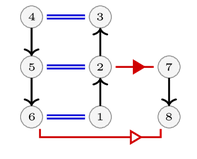
\includegraphics[scale=1]{rin23_2.png}  
  \caption{RIN n°23}
  \label{fig:sub-first}
\end{subfigure}
\begin{subfigure}{.5\textwidth}
  \centering
  % include second image
  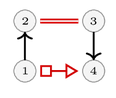
\includegraphics[scale=1]{rin129_2.png}  
  \caption{RIN n°129}
  \label{fig:sub-second}
\end{subfigure}
\end{figure}

La fonction de recherche de motif, \texttt{find\_subgraph}, fonctionne comme ceci : \\
\begin{enumerate}
\item La fonction \texttt{get\_isomorphisms\_vf2} issue de la librairie \texttt{igraph} permet de récupérer la liste de tous les sous-graphes isomorphes entre deux graphes. Ici, on va donc appliquer cette fonction aux graphes g, modélisant une chaîne d'ARN et au motif donné en argument. \\
\item Par ailleurs, pour restreindre la liste des sous-graphes, on va créer une fonction de comparaison des arêtes \texttt{compare\_edges}. Celle-ci va simplement vérifier l'égalité de la couleur des arêtes issues de deux graphes, puis renvoyer le résultat sous forme de booléen.  \\
\item On passe ensuite la fonction \texttt{compare\_edges} en argument à la fonction \texttt{get\_isomorphisms\_vf2}. L'attribut \texttt{edge\_compat\_fn} permet de passer cette fonction de comparaison des arêtes. Pour plus d'informations, voir la documentation de la fonction ici : 
\url{https://igraph.org/python/doc/igraph.GraphBase-class.html#get_isomorphisms_vf2} \\
\item On a donc récupéré ici la liste des sous-graphes correspondant au motif donné, grâce à la vérification de la couleur des arêtes, qui correspondent chacune à un type d'interaction de Leontis-Westhof.
Cependant, il reste encore un problème à résoudre : les doublons. En effet, le programme peut renvoyer le résultat : [[0,1,2,3],[1,0,2,3]].
On voit que les deux sous-graphes sont identiques, les indices ont simplement été déplacés. Pour résoudre ce problème, nous avons utilisé une la structure de données immuable \texttt{frozenset}, afin de stocker temporairement un élément de la liste. En fait, on va itérer sur chacun des éléments de la liste des sous-graphes, et s'assurer qu'aucun n'est identique à l'élement courant. On va ainsi supprimer de nombreux doublons, et donc réduire la taille de la liste des sous-graphes. \\
\item Pour finir, on a donc récupéré la liste des sous-graphes de g, correspondant au RIN passé en argument. Cependant, il reste un point que nous n'avons pas su résoudre. En effet, dans la liste des sous-graphes, il peut y avoir des éléments qui possèdent des noeuds en commun. Par exemple, on peut avoir : [[0,1,2,3],[2,3,4,5]]. Cela a pour conséquence, lorsque l'on calcule le nombre de RIN sur tous les fichiers, qu'on a un nombre très important de motifs trouvés, comparé à celui attendu sur Carnaval. Cela est normal, étant donné qu'on détecte parfois des motifs passant par un noeud identique. Il aurait dans l'idéal fallu être plus restrictif vis à vis de la détection de motif (aucun noeuds en commun pour deux motifs différents), mais nous n'avons malheureusement pas su mettre en oeuvre cette solution.

\end{enumerate}
Pour illustrer le propos, voici le résultat de l'exécution de la version multithreadée du projet (commande \texttt{python projet\_multithread.py}) :
\begin{figure}[!h]
\centering 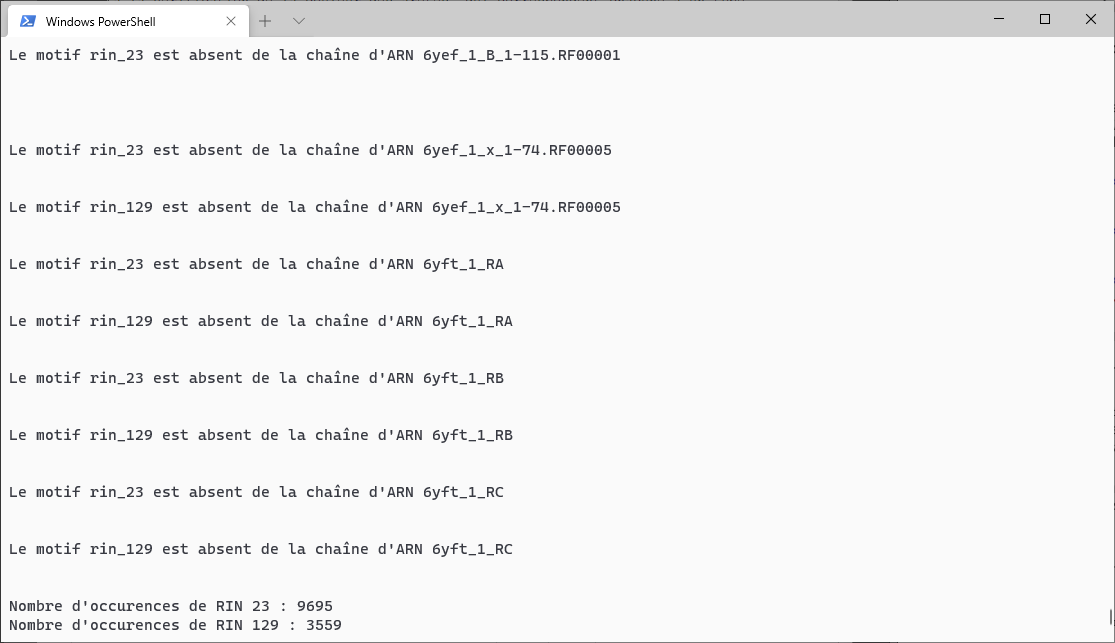
\includegraphics[scale=0.6]{screenshot.png}
\caption{Résultat de la commande \texttt{python projet\_multithread.py}}
\end{figure}

À titre d'information, cette commande a mis environ 7 min à s'exécuter sur une machine dotée de 6 coeurs et 12 threads et environ 20 min sur une machine dotée de 4 coeurs et 8 threads. Il faut donc prévoir selon la configuration de votre machine de quelques minutes à quelques dizaines de minutes pour l'exécution du programme.

\section{Conclusion}
Pour conclure ce rapport, nous allons faire un point sur ce que nous avons réussi à implémenter par rapport aux consignes ainsi que les points d'amélioration.\\
\begin{itemize}
\item Modélisation sous forme de graphe d'une chaîne d'ARN stockée au format CSV. Une amélioration possible consisterait à encadrer sur le dessin du graphe les motifs trouvés, avec des carrés rouge et vert, correspondant respectivement au RIN 23 et 129. 
\item Détection des motifs RIN, bien qu'encore améliorable. Il reste à supprimer les sous-graphes partageant au moins un noeud en commun, pour réduire la taille de la liste des sous-graphes.
\item Parcours de l'ensemble des fichiers et calcul du nombre de RIN. Nous avons d'ailleurs constaté que ce calcul prenait beaucoup de temps sur un seul thread, c'est pour cela qu'une seconde version parallélisée du programme, nommée \texttt{projet\_multithread.py}, est disponible. Vous constatez un grand nombre de RIN détéctés (plusieurs milliers), ce qui est logique vu le problème des noeuds partagés entre sous-graphes, comme évoqué précédemment.
\end{itemize}

\end{document}
 